\documentclass{beamer}
\usepackage{tikz}
\usetikzlibrary{calc,patterns,angles,quotes,shapes,math,decorations,
                through,intersections,lindenmayersystems,backgrounds}
\usepackage{circuitikz}                                                 % draw circuits    
\usepackage{pgfplots}
\usepackage{pgfplots}	
%
%	more math stuff
%
\usepackage{amsmath,amsfonts,amssymb,amsthm}
\usepackage{mathtools}
\usepackage{commath}                                                    % get \norm{x}
\usepackage{fixmath}                                                    % get \mathbold
\usepackage{gensymb}                                                    % get \degree
\usepackage{mathrsfs}
\usepackage{hyperref}
\usepackage{subcaption}
% \usepackage{authblk}													% stops \author{} from working in beamer
\usepackage{graphicx}
\usepackage{hyperref}
\usepackage{alltt}
\usepackage{xcolor}
\usepackage{ifthen}
\usepackage{float}
\usepackage{braket}
\usepackage{siunitx}
\usepackage{relsize}
\usepackage{multirow}
\usepackage{esvect}
\usepackage{setspace}

\usepackage{changepage} % needed for adjustwidth
%
%	beamer stuff
%
% \usetheme[titleformat=smallcaps,block=fill]{metropolis}
%%\metroset{outer/frametitleformat=smallcaps}
% \setbeamertemplate{navigation symbols}{}
% \setbeamertemplate{blocks}[rounded]

% Theme choice:
\usetheme{CambridgeUS}

% Title page details: 
\title{Using the CambridgeUS beamer theme}
\subtitle{Some Tests}
\author{David Meyer}
\institute{Mos Eisley Spaceport}
\date{\today}
\logo{\large \LaTeX{}}
%
%
%
\begin{document} 

% Title page frame
\begin{frame}
    \titlepage 
\end{frame}

% Remove logo from the next slides
\logo{}


% Outline frame
% \begin{frame}{Outline}
%   \tableofcontents
% \end{frame}



\begin{frame}
\frametitle{The Brachistochrone Problem}
%
%	brachistochrone problem setup 
%

%
%	Match beamer theme colors
%
% \usebeamercolor{palette tertiary}

\begin{center}
     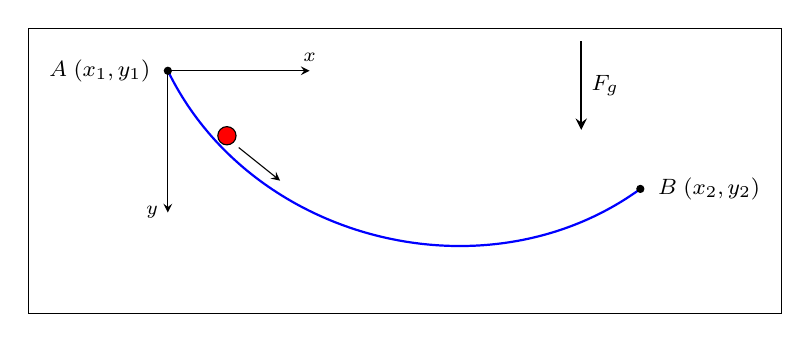
\begin{tikzpicture} [framed,scale=1.50]                            % draw the picture inside a black frame (requires \usetikzlibrary{backgrounds})
%
%	set up some coordinates
%
        \coordinate (A)		at (0.0,  0.0);								% put the origin at A
        \coordinate (Ax)	at (1.2,  0.0);								% x axis here
        \coordinate (Ay)	at (0.0, -1.2);								% y axis positive in the down direction
        \coordinate (Ball)	at (0.5, -0.55);							% draw the ball here
        \coordinate (B)		at (4.0, -1.0);								% other end of the curve
        \coordinate (Gy0)	at (3.5,  0.25);							% draw the gravity vector starting here
        \coordinate (Gy1)	at (3.5, -0.5);								% gravity vector ends here
        \coordinate (D0)	at (0.60,-0.65);							% draw motion arrow starting here
        \coordinate (D1)	at (0.95,-0.93);							% motion arrow ends here
%
%	draw the picture
%
        \draw[blue, thick] (A) to [bend right=50] (B);                 	% draw the curve in blue
% 		\fill [palette tertiary.bg,draw=black] (Ball) circle [radius=0.83mm];	% match beamer theme colors
        \node[circle, draw=black, fill=red, scale=0.70] at (Ball) {};	% draw a red ball with a black outline on the curve
        \draw[-stealth, thin] (D0) -- (D1);								% draw an arrow in the direction the ball is moving
        \fill (A) circle (0.035);										% put a dot on the curve at A
        \fill (B) circle (0.035);										% put a dot on the curve at B
        \draw[draw=none] (A) node[xshift=-0.10cm, font=\footnotesize, left] {$A \; (x_1,y_1)$};		% label A
        \draw[draw=none] (B) node[xshift=0.10cm, font=\footnotesize, right] {$B \; (x_2,y_2)$};		% label B
        \draw[-stealth, thin] (A) -- (Ax) coordinate [label={[font=\scriptsize, above] $x$}];		% draw x axis
        \draw[-stealth, thin] (A) -- (Ay) coordinate [label={[font=\scriptsize, left] $y$}];		% draw y axis
        \draw[-stealth, thick] (Gy0) -- (Gy1) coordinate [label={[font=\footnotesize, midway, right] $\vv{F_{g}}$}];	% draw the gravity vector (g)
      \end{tikzpicture}													% end \tikzipcture
\end{center}
%
%
%
\vspace{0.5cm}
\begin{small}
{\setstretch{1.25}
Given two points $A$ and $B$ in a vertical plane, what is the curve traced 
out by a point acted on only by gravity, which starts at $A$ and reaches 
$B$ in the shortest time?
\par}
\end{small}
\end{frame}



\begin{frame}
\frametitle{A Few Algebraic Structures}
\vspace{-2.0cm}

% \begin{adjustwidth}{-3.25em}{-2.0em} % left justify the table a bit
\begin{center}
\begin{table}
\scalebox{0.55}{
\begin{tabular}{l|c|c|c|c|c|c}
{{\large \bf Structure}}        & $\textbf{\large ABO}$                & {\large \bf Identity}
                                & {\large \bf Inverse}                 & {\large \bf $\text{Distributive}$}
                                & {\large\bf $\text{Commutative}$}     & {\bf Comments} \\
\hline\hline					% separate column names from rows
Semigroup                       & \checkmark & no         & no         & N/A        & no    & $(S,\circ)$ \\
Monoid                          & \checkmark & \checkmark & no         & N/A        & no    & Semigroup plus identity $\in S$ \\
Group                           & \checkmark & \checkmark & \checkmark & N/A        & no    & Monoid plus inverse $\in S$ \\
Abelian Group                   & \checkmark & \checkmark & \checkmark & N/A        & \checkmark $(\circ)$ & Commutative group \\
$\text{Ring}_{+}$               & \checkmark & \checkmark & \checkmark & \checkmark & \checkmark $(+)$     & Abelian group under $+$ \\
$\text{Ring}_{*}$               & \checkmark & yes/no     & no         & \checkmark & no                   & Monoid under $*$ \\
$\text{Field}_{(+,*)}$          & \checkmark & \checkmark $(+,*)$      & \checkmark $(+,*)$ & \checkmark   & \checkmark $(+,*)$
                                             & Abelian group under $+$ and $*$  \\
Vector Space                    & \checkmark & \checkmark $(+,*)$      & \checkmark $(+)$   & \checkmark   & \checkmark $(+)$
                                             & Abelian group under $+$, scalars $\in$ Field \\
Module		                	& \checkmark & \checkmark $(+,*)$          & \checkmark $(+)$   & \checkmark   & \checkmark $(+)$
                                             & Abelian group under $+$, scalars $\in$ Ring

\end{tabular}}
\end{table}
\end{center}
% \end{adjustwidth}
\end{frame}



\begin{frame}
\frametitle{What Are Prime Numbers?}
\begin{definition}
A \alert{prime number} is a number that has exactly two divisors.
\end{definition}
\begin{example}
\begin{itemize}
\item 2 is prime (two divisors: 1 and 2).
\item 3 is prime (two divisors: 1 and 3).
\item 4 is not prime (\alert{three} divisors: 1, 2, and 4).
\end{itemize}
\end{example}
\end{frame}

\end{document} 

